\chapter{Umsetzung}
In diesem Kapitel werden die wichtigsten Klassen und deren Funktionsweisen erläutert. Jede Klasse wird kurz beschrieben, wobei der Fokus auf ihrer Rolle im Gesamtsystem und ihrer Implementierung liegt.

\section{Klassenübersicht}
Das Klassendiagramm zeigt die Beziehungen der wichtigsten Komponenten des Rubik's Cube Projekts. Die Basis bildet das Interface \texttt{IGameInterface}, das von \texttt{RubiksGameInterface} implementiert wird. Diese zentrale Klasse koordiniert das Zusammenspiel von Eingaben (\texttt{InputSystem}, unterstützt durch \texttt{KeyboardObserver}), der Logik (\texttt{RubiksCube}) und der Darstellung (\texttt{CubieRenderer}).

Der Würfel selbst besteht aus \texttt{Cubie}-Objekten, die von \texttt{RubiksCube} organisiert werden. Zur Unterstützung von Rendering-Aufgaben wird die Klasse \texttt{ShaderUtil} genutzt, welche die Shader-Verwaltung übernimmt. Abbildung \ref{SimpleClassDia} verdeutlicht die Beziehungen der Klassen.

\begin{figure} [H]
	\centering
	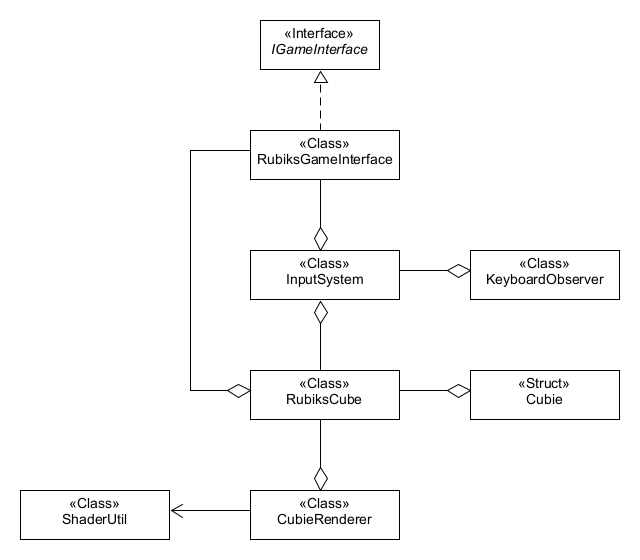
\includegraphics[scale=0.6]{images/SimpleClassDia.png}
	\caption{Vereinfachtes Klassendiagramm}
	\label{SimpleClassDia}
\end{figure}

\section{main.cpp}
Der Code in \texttt{main.cpp} dient als Einstiegspunkt des Projekts. Hier wird \textit{GLFW} initialisiert, ein Fenster erstellt und die \textit{GLEW}-Bibliothek geladen, um moderne OpenGL-Funktionen nutzen zu können. Ein Objekt vom Typ \texttt{RubiksGameInterface} wird erstellt und als aktuelle Schnittstelle festgelegt. Der Game-Loop verarbeitet Benutzereingaben und rendert das Fenster. Ein zusätzlicher Mechanismus stellt sicher, dass das Programm bei minimiertem Fenster nicht abstürzt. Nach dem Schließen des Fensters werden mit der Methode \texttt{ShutdownSystem()} alle Ressourcen freigegeben und \textit{GLFW} ordnungsgemäß beendet.


\section{RubiksGameInterface und IGameInterface}
Die Klasse \texttt{RubiksGameInterface} implementiert das Interface \texttt{IGameInterface} und stellt die zentrale Schnittstelle für die Verwaltung des Spiels dar.
Die Methode \texttt{Initialize(GLFWwindow* window)} kümmert sich um die Initialisierung des Spielfensters und des Eingabesystems. Dabei wird das Fensterobjekt in \texttt{m\_window} gespeichert und das Eingabesystem durch den Aufruf von \texttt{m\_input.Initialize(window)} eingerichtet. Der Rubik's Cube wird durch \texttt{m\_rubiksCube.Initialize(*this)} initialisiert. Zusätzlich wird mit \texttt{m\_input.ObserverKey(GLFW\_KEY\_SPACE)} ein Observer für die Leertaste erstellt.

Die Methode \texttt{Render(float aspectRatio)} ist für das Zeichnen des Fensters und des Rubik's Cube verantwortlich. Sie berechnet bei Bedarf die Projektions- und View-Matrizen neu, wenn die Kameraposition oder das Seitenverhältnis des Fensters sich geändert haben. Anschließend wird die Renderlogik auf den Rubik's Cube angewendet, um dessen aktuellen Zustand mit dem Aufruf von \texttt{m\_rubiksCube.Render(m\_projection * m\_view)} darzustellen.

Die Methode \texttt{Update(double deltaTime)} verarbeitet die Benutzereingaben und aktualisiert den Rubik's Cube. Wenn die Leertaste gedrückt wird, erfolgt ein Zurücksetzen des Rubik's Cubes, andernfalls wird \texttt{m\_rubiksCube.Update(*this)} aufgerufen. Änderungen der Kameraentfernung, die durch das Mausrad bedingt sind, werden in Echtzeit aktualisiert, indem der Wert von \texttt{m\_CameraDistance} angepasst wird. Der Kameraabstand wird durch \texttt{if}-Abfragen auf bestimmte Werte begrenzt. Die Methode \texttt{ClearResources()} gibt die Ressourcen des \texttt{m\_rubiksCube}-Objektes frei.

Zusätzlich verfügt die Klasse über die Methode \texttt{QueueMatrixRecalculation()}, die es ermöglicht, das Neuberechnen der Projektions- und View-Matrizen gezielt anzustoßen.
Weitere Getter-Methoden erlauben den Zugriff auf \texttt{m\_deltaTime} und \texttt{m\_input}. 

Abbildung \ref{RubiksGameInterfaceDia} zeigt das Klassendiagramm zu diesem Abschnitt.

\begin{figure} [H]
	\centering
	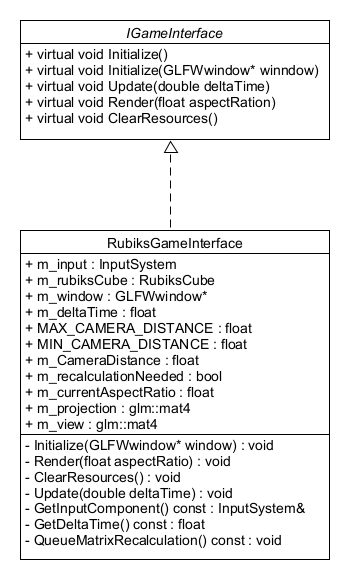
\includegraphics[scale=0.6]{images/GameInterfaceClassDia.png}
	\caption{Klassendiagramm RubiksGameInterface}
	\label{RubiksGameInterfaceDia}
\end{figure}

\section{InputSystem und KeyboardObserver}

\section{CubieRenderer und ShaderUtil}

\section{RubiksCube und Cubie}
